
%% L3-project-paper-template.tex
%% v1.1
%% Dec, 2022
%% Craig Stewart
%% for Durham University, Computer Science Project paper templates
%% contact craig.d.stewart at durham.ac.uk for support
%%
%% Based on IEEE Template: bare_jrnl_compsoc.tex, V1.4b, by Michael Shell
%%
%% Notice from original IEEE Template:
%%*************************************************************************
%% Legal Notice:
%% This code is offered as-is without any warranty either expressed or
%% implied; without even the implied warranty of MERCHANTABILITY or
%% FITNESS FOR A PARTICULAR PURPOSE! 
%% User assumes all risk.
%% In no event shall the IEEE or any contributor to this code be liable for
%% any damages or losses, including, but not limited to, incidental,
%% consequential, or any other damages, resulting from the use or misuse
%% of any information contained here.
%%
%% All comments are the opinions of their respective authors and are not
%% necessarily endorsed by the IEEE.
%%
%% This work is distributed under the LaTeX Project Public License (LPPL)
%% ( http://www.latex-project.org/ ) version 1.3, and may be freely used,
%% distributed and modified. A copy of the LPPL, version 1.3, is included
%% in the base LaTeX documentation of all distributions of LaTeX released
%% 2003/12/01 or later.
%% Retain all contribution notices and credits.
%% ** Modified files should be clearly indicated as such, including  **
%% ** renaming them and changing author support contact information. **
%%*************************************************************************


\documentclass[10pt,journal,compsoc]{IEEEtran}

% Some very useful LaTeX packages include:
% (uncomment the ones you want to load)


%% ---------------------------------------------- START OF USEFUL PACKAGES ----------------------------------------------

%\usepackage{ifpdf}
% Heiko Oberdiek's ifpdf.sty is very useful if you need conditional
% compilation based on whether the output is pdf or dvi.
% usage:
% \ifpdf
%   % pdf code
% \else
%   % dvi code
% \fi
% The latest version of ifpdf.sty can be obtained from:
% http://www.ctan.org/pkg/ifpdf
% Also, note that IEEEtran.cls V1.7 and later provides a builtin
% \ifCLASSINFOpdf conditional that works the same way.
% When switching from latex to pdflatex and vice-versa, the compiler may
% have to be run twice to clear warning/error messages.


% *** CITATION PACKAGES ***
%
\ifCLASSOPTIONcompsoc
  % IEEE Computer Society needs nocompress option
  % requires cite.sty v4.0 or later (November 2003)
  \usepackage[nocompress]{cite}
\else
  % normal IEEE
  \usepackage{cite}
\fi
% cite.sty was written by Donald Arseneau
% V1.6 and later of IEEEtran pre-defines the format of the cite.sty package
% \cite{} output to follow that of the IEEE. Loading the cite package will
% result in citation numbers being automatically sorted and properly
% "compressed/ranged". e.g., [1], [9], [2], [7], [5], [6] without using
% cite.sty will become [1], [2], [5]--[7], [9] using cite.sty. cite.sty's
% \cite will automatically add leading space, if needed. Use cite.sty's
% noadjust option (cite.sty V3.8 and later) if you want to turn this off
% such as if a citation ever needs to be enclosed in parenthesis.
% cite.sty is already installed on most LaTeX systems. Be sure and use
% version 5.0 (2009-03-20) and later if using hyperref.sty.
% The latest version can be obtained at:
% http://www.ctan.org/pkg/cite
% The documentation is contained in the cite.sty file itself.
%
% Note that some packages require special options to format as the Computer
% Society requires. In particular, Computer Society  papers do not use
% compressed citation ranges as is done in typical IEEE papers
% (e.g., [1]-[4]). Instead, they list every citation separately in order
% (e.g., [1], [2], [3], [4]). To get the latter we need to load the cite
% package with the nocompress option which is supported by cite.sty v4.0
% and later. Note also the use of a CLASSOPTION conditional provided by
% IEEEtran.cls V1.7 and later.


% *** GRAPHICS RELATED PACKAGES ***
%
\ifCLASSINFOpdf
  \usepackage[pdftex]{graphicx}
  % declare the path(s) where your graphic files are
  % \graphicspath{{../pdf/}{../jpeg/}}
  % and their extensions so you won't have to specify these with
  % every instance of \includegraphics
  % \DeclareGraphicsExtensions{.pdf,.jpeg,.png}
\else
  % or other class option (dvipsone, dvipdf, if not using dvips). graphicx
  % will default to the driver specified in the system graphics.cfg if no
  % driver is specified.
  % \usepackage[dvips]{graphicx}
  % declare the path(s) where your graphic files are
  % \graphicspath{{../eps/}}
  % and their extensions so you won't have to specify these with
  % every instance of \includegraphics
  % \DeclareGraphicsExtensions{.eps}
\fi
% graphicx was written by David Carlisle and Sebastian Rahtz. It is
% required if you want graphics, photos, etc. graphicx.sty is already
% installed on most LaTeX systems. The latest version and documentation
% can be obtained at: 
% http://www.ctan.org/pkg/graphicx
% Another good source of documentation is "Using Imported Graphics in
% LaTeX2e" by Keith Reckdahl which can be found at:
% http://www.ctan.org/pkg/epslatex
%
% latex, and pdflatex in dvi mode, support graphics in encapsulated
% postscript (.eps) format. pdflatex in pdf mode supports graphics
% in .pdf, .jpeg, .png and .mps (metapost) formats. Users should ensure
% that all non-photo figures use a vector format (.eps, .pdf, .mps) and
% not a bitmapped formats (.jpeg, .png). The IEEE frowns on bitmapped formats
% which can result in "jaggedy"/blurry rendering of lines and letters as
% well as large increases in file sizes.
%
% You can find documentation about the pdfTeX application at:
% http://www.tug.org/applications/pdftex


% *** MATH PACKAGES ***
%
%\usepackage{amsmath}
% A popular package from the American Mathematical Society that provides
% many useful and powerful commands for dealing with mathematics.
%
% Note that the amsmath package sets \interdisplaylinepenalty to 10000
% thus preventing page breaks from occurring within multiline equations. Use:
%\interdisplaylinepenalty=2500
% after loading amsmath to restore such page breaks as IEEEtran.cls normally
% does. amsmath.sty is already installed on most LaTeX systems. The latest
% version and documentation can be obtained at:
% http://www.ctan.org/pkg/amsmath


% *** SPECIALIZED LIST PACKAGES ***
%
%\usepackage{algorithmic}
% algorithmic.sty was written by Peter Williams and Rogerio Brito.
% This package provides an algorithmic environment fo describing algorithms.
% You can use the algorithmic environment in-text or within a figure
% environment to provide for a floating algorithm. Do NOT use the algorithm
% floating environment provided by algorithm.sty (by the same authors) or
% algorithm2e.sty (by Christophe Fiorio) as the IEEE does not use dedicated
% algorithm float types and packages that provide these will not provide
% correct IEEE style captions. The latest version and documentation of
% algorithmic.sty can be obtained at:
% http://www.ctan.org/pkg/algorithms
% Also of interest may be the (relatively newer and more customizable)
% algorithmicx.sty package by Szasz Janos:
% http://www.ctan.org/pkg/algorithmicx


% *** ALIGNMENT PACKAGES ***
%
%\usepackage{array}
% Frank Mittelbach's and David Carlisle's array.sty patches and improves
% the standard LaTeX2e array and tabular environments to provide better
% appearance and additional user controls. As the default LaTeX2e table
% generation code is lacking to the point of almost being broken with
% respect to the quality of the end results, all users are strongly
% advised to use an enhanced (at the very least that provided by array.sty)
% set of table tools. array.sty is already installed on most systems. The
% latest version and documentation can be obtained at:
% http://www.ctan.org/pkg/array


% IEEEtran contains the IEEEeqnarray family of commands that can be used to
% generate multiline equations as well as matrices, tables, etc., of high
% quality.


% *** SUBFIGURE PACKAGES ***
%\ifCLASSOPTIONcompsoc
%  \usepackage[caption=false,font=footnotesize,labelfont=sf,textfont=sf]{subfig}
%\else
%  \usepackage[caption=false,font=footnotesize]{subfig}
%\fi
% subfig.sty, written by Steven Douglas Cochran, is the modern replacement
% for subfigure.sty, the latter of which is no longer maintained and is
% incompatible with some LaTeX packages including fixltx2e. However,
% subfig.sty requires and automatically loads Axel Sommerfeldt's caption.sty
% which will override IEEEtran.cls' handling of captions and this will result
% in non-IEEE style figure/table captions. To prevent this problem, be sure
% and invoke subfig.sty's "caption=false" package option (available since
% subfig.sty version 1.3, 2005/06/28) as this is will preserve IEEEtran.cls
% handling of captions.
% Note that the Computer Society format requires a sans serif font rather
% than the serif font used in traditional IEEE formatting and thus the need
% to invoke different subfig.sty package options depending on whether
% compsoc mode has been enabled.
%
% The latest version and documentation of subfig.sty can be obtained at:
% http://www.ctan.org/pkg/subfig


% *** FLOAT PACKAGES ***
%
%\usepackage{fixltx2e}
% fixltx2e, the successor to the earlier fix2col.sty, was written by
% Frank Mittelbach and David Carlisle. This package corrects a few problems
% in the LaTeX2e kernel, the most notable of which is that in current
% LaTeX2e releases, the ordering of single and double column floats is not
% guaranteed to be preserved. Thus, an unpatched LaTeX2e can allow a
% single column figure to be placed prior to an earlier double column
% figure.
% Be aware that LaTeX2e kernels dated 2015 and later have fixltx2e.sty's
% corrections already built into the system in which case a warning will
% be issued if an attempt is made to load fixltx2e.sty as it is no longer
% needed.
% The latest version and documentation can be found at:
% http://www.ctan.org/pkg/fixltx2e

%\usepackage{stfloats}
% stfloats.sty was written by Sigitas Tolusis. This package gives LaTeX2e
% the ability to do double column floats at the bottom of the page as well
% as the top. (e.g., "\begin{figure*}[!b]" is not normally possible in
% LaTeX2e). It also provides a command:
%\fnbelowfloat
% to enable the placement of footnotes below bottom floats (the standard
% LaTeX2e kernel puts them above bottom floats). This is an invasive package
% which rewrites many portions of the LaTeX2e float routines. It may not work
% with other packages that modify the LaTeX2e float routines. The latest
% version and documentation can be obtained at:
% http://www.ctan.org/pkg/stfloats
% Do not use the stfloats baselinefloat ability as the IEEE does not allow
% \baselineskip to stretch. Authors submitting work to the IEEE should note
% that the IEEE rarely uses double column equations and that authors should try
% to avoid such use. Do not be tempted to use the cuted.sty or midfloat.sty
% packages (also by Sigitas Tolusis) as the IEEE does not format its papers in
% such ways.
% Do not attempt to use stfloats with fixltx2e as they are incompatible.
% Instead, use Morten Hogholm'a dblfloatfix which combines the features
% of both fixltx2e and stfloats:
%
% \usepackage{dblfloatfix}
% The latest version can be found at:
% http://www.ctan.org/pkg/dblfloatfix


%\ifCLASSOPTIONcaptionsoff
%  \usepackage[nomarkers]{endfloat}
% \let\MYoriglatexcaption\caption
% \renewcommand{\caption}[2][\relax]{\MYoriglatexcaption[#2]{#2}}
%\fi
% endfloat.sty was written by James Darrell McCauley, Jeff Goldberg and 
% Axel Sommerfeldt. This package may be useful when used in conjunction with 
% IEEEtran.cls'  captionsoff option. Some IEEE journals/societies require that
% submissions have lists of figures/tables at the end of the paper and that
% figures/tables without any captions are placed on a page by themselves at
% the end of the document. If needed, the draftcls IEEEtran class option or
% \CLASSINPUTbaselinestretch interface can be used to increase the line
% spacing as well. Be sure and use the nomarkers option of endfloat to
% prevent endfloat from "marking" where the figures would have been placed
% in the text. The two hack lines of code above are a slight modification of
% that suggested by in the endfloat docs (section 8.4.1) to ensure that
% the full captions always appear in the list of figures/tables - even if
% the user used the short optional argument of \caption[]{}.
% IEEE papers do not typically make use of \caption[]'s optional argument,
% so this should not be an issue. A similar trick can be used to disable
% captions of packages such as subfig.sty that lack options to turn off
% the subcaptions:
% For subfig.sty:
% \let\MYorigsubfloat\subfloat
% \renewcommand{\subfloat}[2][\relax]{\MYorigsubfloat[]{#2}}
% However, the above trick will not work if both optional arguments of
% the \subfloat command are used. Furthermore, there needs to be a
% description of each subfigure *somewhere* and endfloat does not add
% subfigure captions to its list of figures. Thus, the best approach is to
% avoid the use of subfigure captions (many IEEE journals avoid them anyway)
% and instead reference/explain all the subfigures within the main caption.
% The latest version of endfloat.sty and its documentation can obtained at:
% http://www.ctan.org/pkg/endfloat
%
% The IEEEtran \ifCLASSOPTIONcaptionsoff conditional can also be used
% later in the document, say, to conditionally put the References on a 
% page by themselves.


% *** PDF, URL AND HYPERLINK PACKAGES ***
%
%\usepackage{url}
% url.sty was written by Donald Arseneau. It provides better support for
% handling and breaking URLs. url.sty is already installed on most LaTeX
% systems. The latest version and documentation can be obtained at:
% http://www.ctan.org/pkg/url
% Basically, \url{my_url_here}.

%% ---------------------------------------------- END OF USEFUL PACKAGES ----------------------------------------------



% *** Do not adjust lengths that control margins, column widths, etc. ***
% *** Do not use packages that alter fonts (such as pslatex).         ***

% correct bad hyphenation here
\hyphenation{op-tical net-works semi-conduc-tor}


\begin{document}
%
% paper title
% Titles are generally capitalized except for words such as a, an, and, as,
% at, but, by, for, in, nor, of, on, or, the, to and up, which are usually
% not capitalized unless they are the first or last word of the title.
% Linebreaks \\ can be used within to get better formatting as desired.
% Do not put math or special symbols in the title.
\title{Surveying the (loss) landscape: using machine learning to improve household survey accuracy}
%
%
% author  

\author{Student Name: Nikhil Woodruff\\Supervisor Name: Professor Iain Stewart\\
Submitted as part of the degree of BSc Computer Science to the\\
Board of Examiners in the Department of Computer Sciences, Durham University
}


% The paper headers
\markboth{DURHAM UNIVERSITY, DEPARTMENT OF COMPUTER SCIENCE}%
{Shell \MakeLowercase{\textit{et al.}}}

\IEEEtitleabstractindextext{%
\begin{abstract}
Microsimulation over survey datasets remains the dominant method for analysing and predicting the impact of government policy. However, the accuracy of these models is often limited by the quality of the survey data. In this paper, I present a novel approach to improving the accuracy of survey data by using machine learning to counter both sampling and measurement error. I evaluate this approach on the UK's Family Resources Survey in combination with other datasets, and benchmark its performance against other state-of-the-art methods including percentile adjustment. I find that the proposed approach is able to improve the accuracy of the survey data as a predictor of more trustworthy statistics from administrative sources (which are not granular enough to be used for microsimulation).
\end{abstract}

\begin{IEEEkeywords}
Machine learning, household surveys, microsimulation, survey error, survey weighting
\end{IEEEkeywords}}

%% --------------------------------------------- DO NOT CHANGE ---------------------------------------------

% make the title area
\maketitle


% To allow for easy dual compilation without having to reenter the
% abstract/keywords data, the \IEEEtitleabstractindextext text will
% not be used in maketitle, but will appear (i.e., to be "transported")
% here as \IEEEdisplaynontitleabstractindextext when the compsoc 
% or transmag modes are not selected <OR> if conference mode is selected 
% - because all conference papers position the abstract like regular
% papers do.
\IEEEdisplaynontitleabstractindextext
% \IEEEdisplaynontitleabstractindextext has no effect when using
% compsoc or transmag under a non-conference mode.
% For peer review papers, you can put extra information on the cover
% page as needed:
% \ifCLASSOPTIONpeerreview
% \begin{center} \bfseries EDICS Category: 3-BBND \end{center}
% \fi
%
% For peerreview papers, this IEEEtran command inserts a page break and
% creates the second title. It will be ignored for other modes.
\IEEEpeerreviewmaketitle

\IEEEraisesectionheading{\section{Introduction}\label{sec:introduction}}
% Computer Society journal (but not conference!) papers do something unusual
% with the very first section heading (almost always called "Introduction").
% They place it ABOVE the main text! IEEEtran.cls does not automatically do
% this for you, but you can achieve this effect with the provided
% \IEEEraisesectionheading{} command. Note the need to keep any \label that
% is to refer to the section immediately after \section in the above as
% \IEEEraisesectionheading puts \section within a raised box.

%% --------------------------------------------- DO NOT CHANGE ---------------------------------------------




% The very first letter is a 2 line initial drop letter followed
% by the rest of the first word in caps (small caps for compsoc).
% 
% form to use if the first word consists of a single letter:
% \IEEEPARstart{A}{demo} file is ....
% 
% Here we have the typical use of a "T" for an initial drop letter
% and "HIS" in caps to complete the first word.
\IEEEPARstart{G}{overnments} allocate trillions of dollars every year through mechanisms, such as tax and benefit benefit policy. Decision-making around the design of policies capturing and directing these resources is largely informed by simulated experiments (\emph{microsimulation}) that predict the impact of these policies, or their counterfactuals, on the general population by emulating tax and benefit legislation for respondents in large household surveys.

\subsection{Household surveys}

Statistics agencies around the world collect data on the characteristics of the population through household surveys. As well as serving as an input to government policy evaluation, these data provide detailed insights into the current properties of the UK household sector, informing government publications on poverty, the disposable income distribution and inequality. However, there is evidence to suggest that these surveys are at least partially inaccurate, and this inaccuracy may be more consequential for certain uses of the survey data.

In the United Kingdom, the most comprehensive household survey is the Family Resources Survey (FRS). This survey is collected annually by the Department for Work and Pensions, and includes approximately 20,000 households in a given year. Estimates for population-level features (such as the median income) can be derived using individual weights for household records which indicate how many UK households each respondent is representative of. 

However, despite a weight generation procedure that aims to ensure accurate representation of the UK household sector, prior research has found that the survey does not accurately predict household statistics well at the very-low or very-high ends of the income distribution: benefit aggregates derived from the FRS are around 20\% lower than the in administrative benefit databases, and top income percentiles are lower than than in HMRC's administrative tax database.

There are two ways that a survey can diverge from the reality of the target population: sampling error and measurement error. In the microdata, measurement error arises where the values of individual observations are incorrect (not necessarily through deliberate deceit from survey respondents- question design and integrity checks can influence the accuracy of responses). Sampling error arises where the sample of respondents is not representative of the target population, primarily manifesting as an incorrect weighting of the household records. Both of these sources of error interact with each other: correcting for a missing household subsector can either be achieved by increasing the weight of an existing record or by transforming the values of another record.

Many existing methods for mitigating these types of inaccuracy make heavy use of arbitrary assumptions about the distribution of survey data variables. For example, in correcting for the under-representation of high incomes, a common approach is to match the top income percentiles of a household survey to percentiles from administrative tax datasets. This can achieve exact parity between the two datasets on this very specific target metric, but this introduces significant risk of overfitting: of all the questions that we could ask of the survey data, income percentiles are a small fraction, and other targets could plausibly be thrown off by this adjustment.

This project aims to evaluate a novel use of a combination of machine learning-based techniques to correct for household survey inaccuracy from both sampling and measurement error, and to compare its performance against other state-of-the-art methods. This approach involves using random forest model inference to synthesise new records, and then using gradient descent to minimise a constructed loss function that measures the deviation of the household survey from a large set of official statistics.


\section{Related Work}
This section presents a survey of existing work on the problems that this project addresses. It should be between 2 to 3 pages in length. The rest of this section shows the formats of subsections as well as some general formatting information for tables, figures, references and equations.

\subsection{Main Text}
The font used for the main text should be Palatino and the font size should be 9.5. The first line of all paragraphs should be indented by 0.5cm, except for the first paragraph of each section, subsection, subsubsection etc. (the paragraph immediately after the header) where no indentation is needed.

\subsection{Figures and Tables}
In general, figures and tables should not appear before they are cited. Place figure captions below the figures; place table titles above the tables. If your figure has two parts, for example, include the labels “(a)” and “(b)” as part of the artwork. Please verify that figures and tables you mention in the text actually exist. Make sure that all tables and figures are numbered as shown in Table \ref{table_example} and Figure \ref{fig:my_label} below.

\begin{figure}[!h]
    \centering
    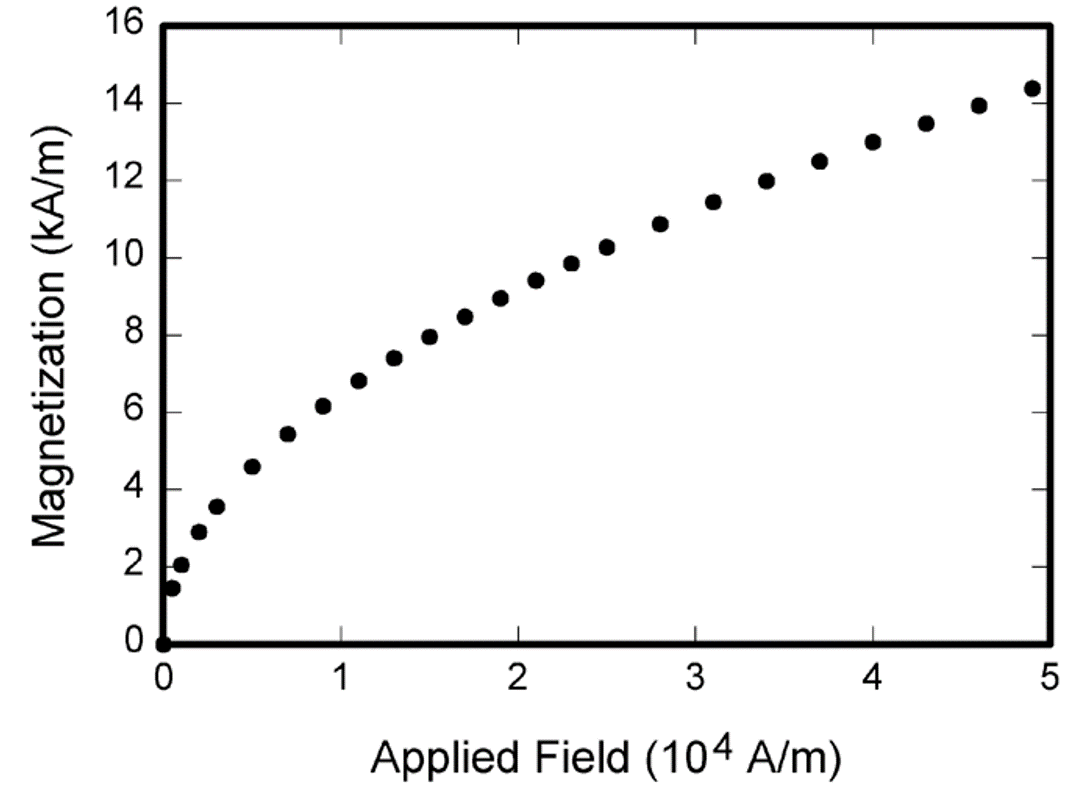
\includegraphics[width=2.5in]{Figure1-template.png}
    \caption{Magnetization as a function of applied field. There is a period after the figure number, followed by two spaces. It is good practice to explain the significance of the figure in the caption}
    \label{fig:my_label}
\end{figure}

% An example of a floating figure using the graphicx package.
% Note that \label must occur AFTER (or within) \caption.
% For figures, \caption should occur after the \includegraphics.
% Note that IEEEtran v1.7 and later has special internal code that
% is designed to preserve the operation of \label within \caption
% even when the captionsoff option is in effect. However, because
% of issues like this, it may be the safest practice to put all your
% \label just after \caption rather than within \caption{}.
%
% Reminder: the "draftcls" or "draftclsnofoot", not "draft", class
% option should be used if it is desired that the figures are to be
% displayed while in draft mode.
%
%\begin{figure}[!h]
%\centering
%\includegraphics[width=2.5in]{myfigure}
%\caption{Simulation results for the network.}
%\label{fig_sim}
%\end{figure}

% An example of a double column floating figure using two subfigures.
% (The subfig.sty package must be loaded for this to work.)
% The subfigure \label commands are set within each subfloat command,
% and the \label for the overall figure must come after \caption.
% \hfil is used as a separator to get equal spacing.
% Watch out that the combined width of all the subfigures on a 
% line do not exceed the text width or a line break will occur.
%
%\begin{figure*}[!t]
%\centering
%\subfloat[Case I]{\includegraphics[width=2.5in]{box}%
%\label{fig_first_case}}
%\hfil
%\subfloat[Case II]{\includegraphics[width=2.5in]{box}%
%\label{fig_second_case}}
%\caption{Simulation results for the network.}
%\label{fig_sim}
%\end{figure*}
%
% Note that often IEEE papers with subfigures do not employ subfigure
% captions (using the optional argument to \subfloat[]), but instead will
% reference/describe all of them (a), (b), etc., within the main caption.
% Be aware that for subfig.sty to generate the (a), (b), etc., subfigure
% labels, the optional argument to \subfloat must be present. If a
% subcaption is not desired, just leave its contents blank,
% e.g., \subfloat[].

\subsection{References}
The list of cited references should appear at the end of the report, listed by order of appearance in the paper. The required style is to note citations in individual brackets, followed by a comma, e.g. “[1], [5]” (as opposed to the more common “[1, 5]” form.) Citation ranges should be formatted as follows: [1], [2], [3], [4] (as opposed to [1]-[4]). When citing a section in a book, please give the relevant page numbers [2]. In sentences, refer simply to the reference number, as in [3]. Do not use “Ref. [3]” or “reference [3]” At the beginning of a sentence use the author names instead of “Reference [3],” e.g., “Smith and Smith [3] show ... .”. 

\section{Methodology}
This section presents the solutions to the problems in detail. The design and implementation details should all be placed in this section. You may create a number of sub-sections, each focusing on one issue.

This section should be between 4 to 6 pages in length.

\begin{table}[!h]
% increase table row spacing, adjust to taste
\caption{Units for Magnetic Properties}
\label{table_example}
\centering
\begin{tabular}{c}
 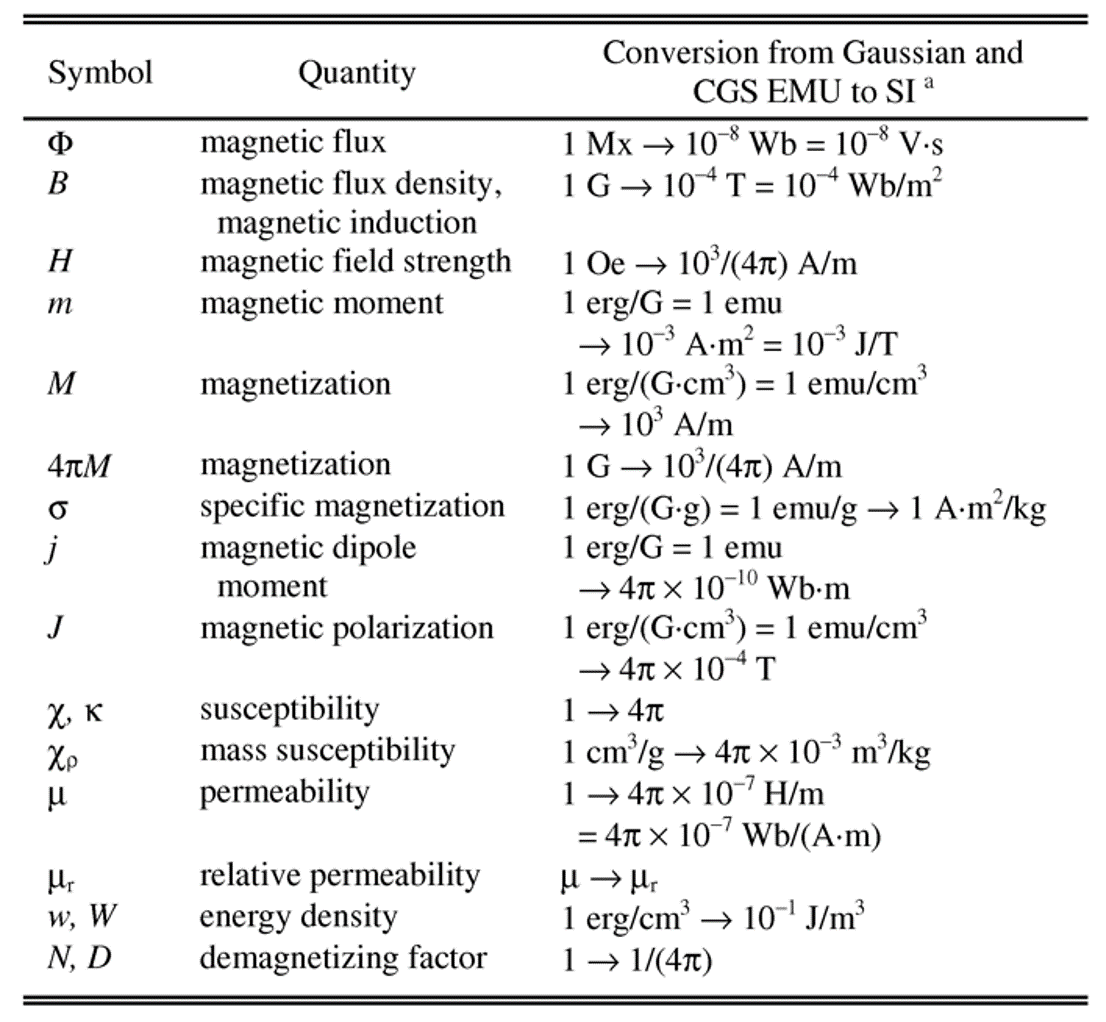
\includegraphics[width=3.5in]{table1.png}
\end{tabular}
\end{table}

% An example of a floating table. Note that, for IEEE style tables, the
% \caption command should come BEFORE the table and, given that table
% captions serve much like titles, are usually capitalized except for words
% such as a, an, and, as, at, but, by, for, in, nor, of, on, or, the, to
% and up, which are usually not capitalized unless they are the first or
% last word of the caption. Table text will default to \footnotesize as
% the IEEE normally uses this smaller font for tables.
% The \label must come after \caption as always.
%
%\begin{table}[!t]
%% increase table row spacing, adjust to taste
%\renewcommand{\arraystretch}{1.3}
% if using array.sty, it might be a good idea to tweak the value of
% \extrarowheight as needed to properly center the text within the cells
%\caption{An Example of a Table}
%\label{table_example}
%\centering
%% Some packages, such as MDW tools, offer better commands for making tables
%% than the plain LaTeX2e tabular which is used here.
%\begin{tabular}{|c||c|}
%\hline
%One & Two\\
%\hline
%Three & Four\\
%\hline
%\end{tabular}
%\end{table}

\noindent \textit{Statements that serve as captions for the entire table do not need footnote letters.  E.g. Mx = maxwell, G = gauss, Oe = oersted; Wb = weber, V = volt, s = second, T = tesla, m = meter, A = ampere, J = joule, kg = kilogram, H = henry.}

\section{Results}
This section presents the results of the solutions. It should include information on experimental settings. The results should demonstrate the claimed benefits/disadvantages of the proposed solutions.

This section should be around 2 pages in length.

\section{Evaluation}
This section should be between 1 to 2 pages in length.

\section{Conclusion}
This section summarises the main points of this paper. Do not replicate the abstract as the conclusion. A conclusion might elaborate on the importance of the work or suggest applications and extensions. This section should be no more than 1 page in length.

The page lengths given for each section are indicative and will vary from project to project but should not exceed the upper limit. A summary is shown in Table \ref{table_2}.

\begin{table}[!t]
\renewcommand{\arraystretch}{1.3}
\caption{Summary of Page Lengths for Sections}
\label{table_2}
\centering
\begin{tabular}{cc}
\hline\hline
Section & Number of Pages\\
\hline
I. Introduction & 2\\
II. Related Work & 2-3\\
III. Methodology & 4-6\\
IV. Results & 2\\
V. Evaluation & 1-2\\
VI. Conclusion & 1\\
\hline\hline
\end{tabular}
\end{table}


% trigger a \newpage just before the given reference
% number - used to balance the columns on the last page
% adjust value as needed - may need to be readjusted if
% the document is modified later
%\IEEEtriggeratref{8}
% The "triggered" command can be changed if desired:
%\IEEEtriggercmd{\enlargethispage{-5in}}

% references section

% can use a bibliography generated by BibTeX as a .bbl file
% BibTeX documentation can be easily obtained at:
% http://mirror.ctan.org/biblio/bibtex/contrib/doc/
% The IEEEtran BibTeX style support page is at:
% http://www.michaelshell.org/tex/ieeetran/bibtex/
%\bibliographystyle{IEEEtran}
% argument is your BibTeX string definitions and bibliography database(s)
%\bibliography{IEEEabrv,../bib/paper}
%
% <OR> manually copy in the resultant .bbl file
% set second argument of \begin to the number of references
% (used to reserve space for the reference number labels box)

\newpage
\begin{thebibliography}{1}

\bibitem{IEEEhowto:bridle}
J.S. Bridle, \emph{Probabilistic Interpretation of Feedforward Classification Network Outputs, with Relationships to Statistical Pattern Recognition}, Neurocomputing—Algorithms, Architectures and Applications, F. Fogelman-Soulie and J. Herault, eds., NATO ASI Series F68, Berlin: Springer-Verlag, pp. 227-236, 1989. (Book style with paper title and editor)

\bibitem{IEEEhowto:chen}
W.-K. Chen, \emph{Linear Networks and Systems}, Belmont, Calif.: Wadsworth, pp. 123-135, 1993. (Book style)

\bibitem{IEEEhowto:poor}
H. Poor, \emph{A Hypertext History of Multiuser Dimensions}, MUD History, http://www.ccs.neu.edu/home/pb/mud-history.html. 1986. (URL link *include year)

\bibitem{IEEEhowto:elissa}
K. Elissa, \emph{An Overview of Decision Theory}, unpublished. (Unpublished manuscript)

\end{thebibliography}

% that's all folks
\end{document}


